\documentclass[nooutcomes]{ximera}

\graphicspath{
  {./}
  {1-1QuantitativeReasoning/}
  {1-2RelationsAndGraphs/}
  {1-3ChangingInTandem/}
  {2-1LinearEquations/}
  {2-2LinearModeling/}
  {2-3ExponentialModeling/}
  {3-1WhatIsAFunction/}
  {3-2FunctionProperties/}
  {3-3AverageRatesOfChange/}
  {4-1BuildingNewFunctions/}
  {4-2Polynomials/}
  {5-1RationalFunctions/}
   {5-2ExponentialFunctions/}
  {6-1Domain/}
  {6-2Range/}
  {6-3CompositionOfFunctions/}
  {6-4FunctionTransformations/}
  {7-1ZerosOfFunctions/}
  {7-XZerosOfPolynomials/}
  {7-2ZerosOfFamousFunctions/}
  {8-1SystemsOfEquations/}
  {6-5FunctionTransformationsProject/}
  {1-1QuantitativeReasoning/exercises/}
  {1-2RelationsAndGraphs/exercises/}
  {../1-3ChangingInTandem/exercises/}
  {../2-1LinearEquations/exercises/}
  {../2-2LinearModeling/exercises/}
  {../2-3ExponentialModeling/exercises/}
  {../3-1WhatIsAFunction/exercises/}
  {../3-2FunctionProperties/exercises/}
  {../3-3AverageRatesOfChange/exercises/}
  {../5-2ExponentialFunctions/exercises/}
  {../4-1BuildingNewFunctions/exercises/}
  {../4-2Polynomials/exercises/}
  {../5-1RationalFunctions/exercises/}
  {../6-1Domain/exercises/}
  {../6-2Range/exercises/}
  {../6-3CompositionOfFunctions/exercises/}
  {../7-1ZerosOfFunctions/exercises/}
  {../7-XZerosOfPolynomials/exercises/}
  {../7-2ZerosOfFamousFunctions/exercises/}
  {../6-4FunctionTransformations/exercises/}
  {../8-1SystemsOfEquations/exercises/}
  {../6-3FunctionTransformationsProject/exercises/}
}

\DeclareGraphicsExtensions{.pdf,.png,.jpg,.eps}

\newcommand{\mooculus}{\textsf{\textbf{MOOC}\textnormal{\textsf{ULUS}}}}

\usepackage[makeroom]{cancel} %% for strike outs

\ifxake
\else
\usepackage[most]{tcolorbox}
\fi


%\typeout{************************************************}
%\typeout{New Environments}
%\typeout{************************************************}

%% to fix for web can be removed when deployed offically with ximera2
\let\image\relax\let\endimage\relax
\NewEnviron{image}{% 
  \begin{center}\BODY\end{center}% center
}



\NewEnviron{folder}{
      \addcontentsline{toc}{section}{\textbf{\BODY}}
}

\ifxake
\let\summary\relax
\let\endsummary\relax
\newtheorem*{summary}{Summary}
\newtheorem*{callout}{Callout}
\newtheorem*{overview}{Overview}
\newtheorem*{objectives}{Objectives}
\newtheorem*{motivatingQuestions}{Motivating Questions}
\newtheorem*{MM}{Metacognitive Moment}
      
%% NEEDED FOR XIMERA 2
%\ximerizedEnvironment{summary}
%\ximerizedEnvironment{callout}
%\ximerizedEnvironment{overview} 
%\ximerizedEnvironment{objectives}
%\ximerizedEnvironment{motivatingQuestions}
%\ximerizedEnvironment{MM}
\else
%% CALLOUT
\NewEnviron{callout}{
  \begin{tcolorbox}[colback=blue!5, breakable,pad at break*=1mm]
      \BODY
  \end{tcolorbox}
}
%% MOTIVATING QUESTIONS
\NewEnviron{motivatingQuestions}{
  \begin{tcolorbox}[ breakable,pad at break*=1mm]
    \textbf{\Large Motivating Questions}\hfill
    %\begin{itemize}[label=\textbullet]
      \BODY
    %\end{itemize}
  \end{tcolorbox}
}
%% OBJECTIVES
\NewEnviron{objectives}{  
    \vspace{.5in}
      %\begin{tcolorbox}[colback=orange!5, breakable,pad at break*=1mm]
    \textbf{\Large Learning Objectives}
    \begin{itemize}[label=\textbullet]
      \BODY
    \end{itemize}
    %\end{tcolorbox}
}
%% DEFINITION
\let\definition\relax
\let\enddefinition\relax
\NewEnviron{definition}{
  \begin{tcolorbox}[ breakable,pad at break*=1mm]
    \noindent\textbf{Definition}~
      \BODY
  \end{tcolorbox}
}
%% OVERVIEW
\let\overview\relax
\let\overview\relax
\NewEnviron{overview}{
  \begin{tcolorbox}[ breakable,pad at break*=1mm]
    \textbf{\Large Overview}
    %\begin{itemize}[label=\textbullet] %% breaks Xake
      \BODY
    %\end{itemize}
  \end{tcolorbox}
}
%% SUMMARY
\let\summary\relax
\let\endsummary\relax
\NewEnviron{summary}{
  \begin{tcolorbox}[ breakable,pad at break*=1mm]
    \textbf{\Large Summary}
    %\begin{itemize}[label=\textbullet] %% breaks Xake
      \BODY
    %\end{itemize}
  \end{tcolorbox}
}
%% REMARK
\let\remark\relax
\let\endremark\relax
\NewEnviron{remark}{
  \begin{tcolorbox}[colback=green!5, breakable,pad at break*=1mm]
    \noindent\textbf{Remark}~
      \BODY
  \end{tcolorbox}
}
%% EXPLANATION
\let\explanation\relax
\let\endexplanation\relax
\NewEnviron{explanation}{
    \normalfont
    \noindent\textbf{Explanation}~
      \BODY
}
%% EXPLORATION
\let\exploration\relax
\let\endexploration\relax
\NewEnviron{exploration}{
  \begin{tcolorbox}[colback=yellow!10, breakable,pad at break*=1mm]
    \noindent\textbf{Exploration}~
      \BODY
  \end{tcolorbox}
}
%% METACOGNITIVE MOMENTS
\let\MM\relax
\let\endMM\relax
\NewEnviron{MM}{
  \begin{tcolorbox}[colback=pink!15, breakable,pad at break*=1mm]
    \noindent\textbf{Metacognitive Moment}~
      \BODY
  \end{tcolorbox}
}


\fi





%Notes on what envirnoment to use:  Example with Explanation in text; if they are supposed to answer- Problem; no answer - Exploration


%\typeout{************************************************}
%% Header and footers
%\typeout{************************************************}

\newcommand{\licenseAcknowledgement}{Licensed under Creative Commons 4.0}
\newcommand{\licenseAPC}{\renewcommand{\licenseAcknowledgement}{\textbf{Acknowledgements:} Active Prelude to Calculus (https://activecalculus.org/prelude) }}
\newcommand{\licenseSZ}{\renewcommand{\licenseAcknowledgement}{\textbf{Acknowledgements:} Stitz Zeager Open Source Mathematics (https://www.stitz-zeager.com/) }}
\newcommand{\licenseAPCSZ}{\renewcommand{\licenseAcknowledgement}{\textbf{Acknowledgements:} Active Prelude to Calculus (https://activecalculus.org/prelude) and Stitz Zeager Open Source Mathematics (https://www.stitz-zeager.com/) }}
\newcommand{\licenseORCCA}{\renewcommand{\licenseAcknowledgement}{\textbf{Acknowledgements:}Original source material, products with readable and accessible
math content, and other information freely available at pcc.edu/orcca.}}
\newcommand{\licenseY}{\renewcommand{\licenseAcknowledgement}{\textbf{Acknowledgements:} Yoshiwara Books (https://yoshiwarabooks.org/)}}
\newcommand{\licenseOS}{\renewcommand{\licenseAcknowledgement}{\textbf{Acknowledgements:} OpenStax College Algebra (https://openstax.org/details/books/college-algebra)}}
\newcommand{\licenseAPCSZCSCC}{\renewcommand{\licenseAcknowledgement}{\textbf{Acknowledgements:} Active Prelude to Calculus (https://activecalculus.org/prelude), Stitz Zeager Open Source Mathematics (https://www.stitz-zeager.com/), CSCC PreCalculus and Calculus texts (https://ximera.osu.edu/csccmathematics)}}

\ifxake\else %% do nothing on the website
\usepackage{fancyhdr}
\pagestyle{fancy}
\fancyhf{}
\fancyhead[R]{\sectionmark}
\fancyfoot[L]{\thepage}
\fancyfoot[C]{\licenseAcknowledgement}
\renewcommand{\headrulewidth}{0pt}
\renewcommand{\footrulewidth}{0pt}
\fi

%%%%%%%%%%%%%%%%



%\typeout{************************************************}
%\typeout{Table of Contents}
%\typeout{************************************************}


%% Edit this to change the font style
\newcommand{\sectionHeadStyle}{\sffamily\bfseries}


\makeatletter

%% part uses arabic numerals
\renewcommand*\thepart{\arabic{part}}


\ifxake\else
\renewcommand\chapterstyle{%
  \def\maketitle{%
    \addtocounter{titlenumber}{1}%
    \pagestyle{fancy}
    \phantomsection
    \addcontentsline{toc}{section}{\textbf{\thepart.\thetitlenumber\hspace{1em}\@title}}%
                    {\flushleft\small\sectionHeadStyle\@pretitle\par\vspace{-1.5em}}%
                    {\flushleft\LARGE\sectionHeadStyle\thepart.\thetitlenumber\hspace{1em}\@title \par }%
                    {\setcounter{problem}{0}\setcounter{sectiontitlenumber}{0}}%
                    \par}}





\renewcommand\sectionstyle{%
  \def\maketitle{%
    \addtocounter{sectiontitlenumber}{1}
    \pagestyle{fancy}
    \phantomsection
    \addcontentsline{toc}{subsection}{\thepart.\thetitlenumber.\thesectiontitlenumber\hspace{1em}\@title}%
    {\flushleft\small\sectionHeadStyle\@pretitle\par\vspace{-1.5em}}%
    {\flushleft\Large\sectionHeadStyle\thepart.\thetitlenumber.\thesectiontitlenumber\hspace{1em}\@title \par}%
    %{\setcounter{subsectiontitlenumber}{0}}%
    \par}}



\renewcommand\section{\@startsection{paragraph}{10}{\z@}%
                                     {-3.25ex\@plus -1ex \@minus -.2ex}%
                                     {1.5ex \@plus .2ex}%
                                     {\normalfont\large\sectionHeadStyle}}
\renewcommand\subsection{\@startsection{subparagraph}{10}{\z@}%
                                    {3.25ex \@plus1ex \@minus.2ex}%
                                    {-1em}%
                                    {\normalfont\normalsize\sectionHeadStyle}}

\fi

%% redefine Part
\renewcommand\part{%
   {\setcounter{titlenumber}{0}}
  \if@openright
    \cleardoublepage
  \else
    \clearpage
  \fi
  \thispagestyle{plain}%
  \if@twocolumn
    \onecolumn
    \@tempswatrue
  \else
    \@tempswafalse
  \fi
  \null\vfil
  \secdef\@part\@spart}

\def\@part[#1]#2{%
    \ifnum \c@secnumdepth >-2\relax
      \refstepcounter{part}%
      \addcontentsline{toc}{part}{\thepart\hspace{1em}#1}%
    \else
      \addcontentsline{toc}{part}{#1}%
    \fi
    \markboth{}{}%
    {\centering
     \interlinepenalty \@M
     \normalfont
     \ifnum \c@secnumdepth >-2\relax
       \huge\sffamily\bfseries \partname\nobreakspace\thepart
       \par
       \vskip 20\p@
     \fi
     \Huge \bfseries #2\par}%
    \@endpart}
\def\@spart#1{%
    {\centering
     \interlinepenalty \@M
     \normalfont
     \Huge \bfseries #1\par}%
    \@endpart}
\def\@endpart{\vfil\newpage
              \if@twoside
               \if@openright
                \null
                \thispagestyle{empty}%
                \newpage
               \fi
              \fi
              \if@tempswa
                \twocolumn
                \fi}



\makeatother





%\typeout{************************************************}
%\typeout{Stuff from Ximera}
%\typeout{************************************************}



\usepackage{array}  %% This is for typesetting long division
\setlength{\extrarowheight}{+.1cm}
\newdimen\digitwidth
\settowidth\digitwidth{9}
\def\divrule#1#2{
\noalign{\moveright#1\digitwidth
\vbox{\hrule width#2\digitwidth}}}





\newcommand{\RR}{\mathbb R}
\newcommand{\R}{\mathbb R}
\newcommand{\N}{\mathbb N}
\newcommand{\Z}{\mathbb Z}

\newcommand{\sagemath}{\textsf{SageMath}}


\def\d{\,d}
%\renewcommand{\d}{\mathop{}\!d}
\newcommand{\dd}[2][]{\frac{\d #1}{\d #2}}
\newcommand{\pp}[2][]{\frac{\partial #1}{\partial #2}}
\renewcommand{\l}{\ell}
\newcommand{\ddx}{\frac{d}{\d x}}



%\newcommand{\unit}{\,\mathrm}
\newcommand{\unit}{\mathop{}\!\mathrm}
\newcommand{\eval}[1]{\bigg[ #1 \bigg]}
\newcommand{\seq}[1]{\left( #1 \right)}
\renewcommand{\epsilon}{\varepsilon}
\renewcommand{\phi}{\varphi}


\renewcommand{\iff}{\Leftrightarrow}

\DeclareMathOperator{\arccot}{arccot}
\DeclareMathOperator{\arcsec}{arcsec}
\DeclareMathOperator{\arccsc}{arccsc}
\DeclareMathOperator{\sign}{sign}


%\DeclareMathOperator{\divergence}{divergence}
%\DeclareMathOperator{\curl}[1]{\grad\cross #1}
\newcommand{\lto}{\mathop{\longrightarrow\,}\limits}

\renewcommand{\bar}{\overline}

\colorlet{textColor}{black}
\colorlet{background}{white}
\colorlet{penColor}{blue!50!black} % Color of a curve in a plot
\colorlet{penColor2}{red!50!black}% Color of a curve in a plot
\colorlet{penColor3}{red!50!blue} % Color of a curve in a plot
\colorlet{penColor4}{green!50!black} % Color of a curve in a plot
\colorlet{penColor5}{orange!80!black} % Color of a curve in a plot
\colorlet{penColor6}{yellow!70!black} % Color of a curve in a plot
\colorlet{fill1}{penColor!20} % Color of fill in a plot
\colorlet{fill2}{penColor2!20} % Color of fill in a plot
\colorlet{fillp}{fill1} % Color of positive area
\colorlet{filln}{penColor2!20} % Color of negative area
\colorlet{fill3}{penColor3!20} % Fill
\colorlet{fill4}{penColor4!20} % Fill
\colorlet{fill5}{penColor5!20} % Fill
\colorlet{gridColor}{gray!50} % Color of grid in a plot

\newcommand{\surfaceColor}{violet}
\newcommand{\surfaceColorTwo}{redyellow}
\newcommand{\sliceColor}{greenyellow}




\pgfmathdeclarefunction{gauss}{2}{% gives gaussian
  \pgfmathparse{1/(#2*sqrt(2*pi))*exp(-((x-#1)^2)/(2*#2^2))}%
}





%\typeout{************************************************}
%\typeout{ORCCA Preamble.Tex}
%\typeout{************************************************}


%% \usepackage{geometry}
%% \geometry{letterpaper,total={408pt,9.0in}}
%% Custom Page Layout Adjustments (use latex.geometry)
%% \usepackage{amsmath,amssymb}
%% \usepackage{pgfplots}
\usepackage{pifont}                                         %needed for symbols, s.a. airplane symbol
\usetikzlibrary{positioning,fit,backgrounds}                %needed for nested diagrams
\usetikzlibrary{calc,trees,positioning,arrows,fit,shapes}   %needed for set diagrams
\usetikzlibrary{decorations.text}                           %needed for text following a curve
\usetikzlibrary{arrows,arrows.meta}                         %needed for open/closed intervals
\usetikzlibrary{positioning,3d,shapes.geometric}            %needed for 3d number sets tower

%% NEEDED FOR XIMERA 1
%\usetkzobj{all}       %NO LONGER VALID
%%%%%%%%%%%%%%

\usepackage{tikz-3dplot}
\usepackage{tkz-euclide}                     %needed for triangle diagrams
\usepgfplotslibrary{fillbetween}                            %shade regions of a plot
\usetikzlibrary{shadows}                                    %function diagrams
\usetikzlibrary{positioning}                                %function diagrams
\usetikzlibrary{shapes}                                     %function diagrams
%%% global colors from https://www.pcc.edu/web-services/style-guide/basics/color/ %%%
\definecolor{ruby}{HTML}{9E0C0F}
\definecolor{turquoise}{HTML}{008099}
\definecolor{emerald}{HTML}{1c8464}
\definecolor{amber}{HTML}{c7502a}
\definecolor{amethyst}{HTML}{70485b}
\definecolor{sapphire}{HTML}{263c53}
\colorlet{firstcolor}{sapphire}
\colorlet{secondcolor}{turquoise}
\colorlet{thirdcolor}{emerald}
\colorlet{fourthcolor}{amber}
\colorlet{fifthcolor}{amethyst}
\colorlet{sixthcolor}{ruby}
\colorlet{highlightcolor}{green!50!black}
\colorlet{graphbackground}{white}
\colorlet{wood}{brown!60!white}
%%% curve, dot, and graph custom styles %%%
\pgfplotsset{firstcurve/.style      = {color=firstcolor,  mark=none, line width=1pt, {Kite}-{Kite}, solid}}
\pgfplotsset{secondcurve/.style     = {color=secondcolor, mark=none, line width=1pt, {Kite}-{Kite}, solid}}
\pgfplotsset{thirdcurve/.style      = {color=thirdcolor,  mark=none, line width=1pt, {Kite}-{Kite}, solid}}
\pgfplotsset{fourthcurve/.style     = {color=fourthcolor, mark=none, line width=1pt, {Kite}-{Kite}, solid}}
\pgfplotsset{fifthcurve/.style      = {color=fifthcolor,  mark=none, line width=1pt, {Kite}-{Kite}, solid}}
\pgfplotsset{highlightcurve/.style  = {color=highlightcolor,  mark=none, line width=5pt, -, opacity=0.3}}   % thick, opaque curve for highlighting
\pgfplotsset{asymptote/.style       = {color=gray, mark=none, line width=1pt, <->, dashed}}
\pgfplotsset{symmetryaxis/.style    = {color=gray, mark=none, line width=1pt, <->, dashed}}
\pgfplotsset{guideline/.style       = {color=gray, mark=none, line width=1pt, -}}
\tikzset{guideline/.style           = {color=gray, mark=none, line width=1pt, -}}
\pgfplotsset{altitude/.style        = {dashed, color=gray, thick, mark=none, -}}
\tikzset{altitude/.style            = {dashed, color=gray, thick, mark=none, -}}
\pgfplotsset{radius/.style          = {dashed, thick, mark=none, -}}
\tikzset{radius/.style              = {dashed, thick, mark=none, -}}
\pgfplotsset{rightangle/.style      = {color=gray, mark=none, -}}
\tikzset{rightangle/.style          = {color=gray, mark=none, -}}
\pgfplotsset{closedboundary/.style  = {color=black, mark=none, line width=1pt, {Kite}-{Kite},solid}}
\tikzset{closedboundary/.style      = {color=black, mark=none, line width=1pt, {Kite}-{Kite},solid}}
\pgfplotsset{openboundary/.style    = {color=black, mark=none, line width=1pt, {Kite}-{Kite},dashed}}
\tikzset{openboundary/.style        = {color=black, mark=none, line width=1pt, {Kite}-{Kite},dashed}}
\tikzset{verticallinetest/.style    = {color=gray, mark=none, line width=1pt, <->,dashed}}
\pgfplotsset{soliddot/.style        = {color=firstcolor,  mark=*, only marks}}
\pgfplotsset{hollowdot/.style       = {color=firstcolor,  mark=*, only marks, fill=graphbackground}}
\pgfplotsset{blankgraph/.style      = {xmin=-10, xmax=10,
                                        ymin=-10, ymax=10,
                                        axis line style={-, draw opacity=0 },
                                        axis lines=box,
                                        major tick length=0mm,
                                        xtick={-10,-9,...,10},
                                        ytick={-10,-9,...,10},
                                        grid=major,
                                        grid style={solid,gray!20},
                                        xticklabels={,,},
                                        yticklabels={,,},
                                        minor xtick=,
                                        minor ytick=,
                                        xlabel={},ylabel={},
                                        width=0.75\textwidth,
                                      }
            }
\pgfplotsset{numberline/.style      = {xmin=-10,xmax=10,
                                        minor xtick={-11,-10,...,11},
                                        xtick={-10,-5,...,10},
                                        every tick/.append style={thick},
                                        axis y line=none,
                                        y=15pt,
                                        axis lines=middle,
                                        enlarge x limits,
                                        grid=none,
                                        clip=false,
                                        axis background/.style={},
                                        after end axis/.code={
                                          \path (axis cs:0,0)
                                          node [anchor=north,yshift=-0.075cm] {\footnotesize 0};
                                        },
                                        every axis x label/.style={at={(current axis.right of origin)},anchor=north},
                                      }
            }
\pgfplotsset{openinterval/.style={color=firstcolor,mark=none,ultra thick,{Parenthesis}-{Parenthesis}}}
\pgfplotsset{openclosedinterval/.style={color=firstcolor,mark=none,ultra thick,{Parenthesis}-{Bracket}}}
\pgfplotsset{closedinterval/.style={color=firstcolor,mark=none,ultra thick,{Bracket}-{Bracket}}}
\pgfplotsset{closedopeninterval/.style={color=firstcolor,mark=none,ultra thick,{Bracket}-{Parenthesis}}}
\pgfplotsset{infiniteopeninterval/.style={color=firstcolor,mark=none,ultra thick,{Kite}-{Parenthesis}}}
\pgfplotsset{openinfiniteinterval/.style={color=firstcolor,mark=none,ultra thick,{Parenthesis}-{Kite}}}
\pgfplotsset{infiniteclosedinterval/.style={color=firstcolor,mark=none,ultra thick,{Kite}-{Bracket}}}
\pgfplotsset{closedinfiniteinterval/.style={color=firstcolor,mark=none,ultra thick,{Bracket}-{Kite}}}
\pgfplotsset{infiniteinterval/.style={color=firstcolor,mark=none,ultra thick,{Kite}-{Kite}}}
\pgfplotsset{interval/.style= {ultra thick, -}}
%%% cycle list of plot styles for graphs with multiple plots %%%
\pgfplotscreateplotcyclelist{pccstylelist}{%
  firstcurve\\%
  secondcurve\\%
  thirdcurve\\%
  fourthcurve\\%
  fifthcurve\\%
}
%%% default plot settings %%%
\pgfplotsset{every axis/.append style={
  axis x line=middle,    % put the x axis in the middle
  axis y line=middle,    % put the y axis in the middle
  axis line style={<->}, % arrows on the axis
  scaled ticks=false,
  tick label style={/pgf/number format/fixed},
  xlabel={$x$},          % default put x on x-axis
  ylabel={$y$},          % default put y on y-axis
  xmin = -7,xmax = 7,    % most graphs have this window
  ymin = -7,ymax = 7,    % most graphs have this window
  domain = -7:7,
  xtick = {-6,-4,...,6}, % label these ticks
  ytick = {-6,-4,...,6}, % label these ticks
  yticklabel style={inner sep=0.333ex},
  minor xtick = {-7,-6,...,7}, % include these ticks, some without label
  minor ytick = {-7,-6,...,7}, % include these ticks, some without label
  scale only axis,       % don't consider axis and tick labels for width and height calculation
  cycle list name=pccstylelist,
  tick label style={font=\footnotesize},
  legend cell align=left,
  grid = both,
  grid style = {solid,gray!20},
  axis background/.style={fill=graphbackground},
}}
\pgfplotsset{framed/.style={axis background/.style ={draw=gray}}}
%\pgfplotsset{framed/.style={axis background/.style ={draw=gray,fill=graphbackground,rounded corners=3ex}}}
%%% other tikz (not pgfplots) settings %%%
%\tikzset{axisnode/.style={font=\scriptsize,text=black}}
\tikzset{>=stealth}
%%% for nested diagram in types of numbers section %%%
\newcommand\drawnestedsets[4]{
  \def\position{#1}             % initial position
  \def\nbsets{#2}               % number of sets
  \def\listofnestedsets{#3}     % list of sets
  \def\reversedlistofcolors{#4} % reversed list of colors
  % position and draw labels of sets
  \coordinate (circle-0) at (#1);
  \coordinate (set-0) at (#1);
  \foreach \set [count=\c] in \listofnestedsets {
    \pgfmathtruncatemacro{\cminusone}{\c - 1}
    % label of current set (below previous nested set)
    \node[below=3pt of circle-\cminusone,inner sep=0]
    (set-\c) {\set};
    % current set (fit current label and previous set)
    \node[circle,inner sep=0,fit=(circle-\cminusone)(set-\c)]
    (circle-\c) {};
  }
  % draw and fill sets in reverse order
  \begin{scope}[on background layer]
    \foreach \col[count=\c] in \reversedlistofcolors {
      \pgfmathtruncatemacro{\invc}{\nbsets-\c}
      \pgfmathtruncatemacro{\invcplusone}{\invc+1}
      \node[circle,draw,fill=\col,inner sep=0,
      fit=(circle-\invc)(set-\invcplusone)] {};
    }
  \end{scope}
  }
\ifdefined\tikzset
\tikzset{ampersand replacement = \amp}
\fi
\newcommand{\abs}[1]{\left\lvert#1\right\rvert}
%\newcommand{\point}[2]{\left(#1,#2\right)}
\newcommand{\highlight}[1]{\definecolor{sapphire}{RGB}{59,90,125} {\color{sapphire}{{#1}}}}
\newcommand{\firsthighlight}[1]{\definecolor{sapphire}{RGB}{59,90,125} {\color{sapphire}{{#1}}}}
\newcommand{\secondhighlight}[1]{\definecolor{emerald}{RGB}{20,97,75} {\color{emerald}{{#1}}}}
\newcommand{\unhighlight}[1]{{\color{black}{{#1}}}}
\newcommand{\lowlight}[1]{{\color{lightgray}{#1}}}
\newcommand{\attention}[1]{\mathord{\overset{\downarrow}{#1}}}
\newcommand{\nextoperation}[1]{\mathord{\boxed{#1}}}
\newcommand{\substitute}[1]{{\color{blue}{{#1}}}}
\newcommand{\pinover}[2]{\overset{\overset{\mathrm{\ #2\ }}{|}}{\strut #1 \strut}}
\newcommand{\addright}[1]{{\color{blue}{{{}+#1}}}}
\newcommand{\addleft}[1]{{\color{blue}{{#1+{}}}}}
\newcommand{\subtractright}[1]{{\color{blue}{{{}-#1}}}}
\newcommand{\multiplyright}[2][\cdot]{{\color{blue}{{{}#1#2}}}}
\newcommand{\multiplyleft}[2][\cdot]{{\color{blue}{{#2#1{}}}}}
\newcommand{\divideunder}[2]{\frac{#1}{{\color{blue}{{#2}}}}}
\newcommand{\divideright}[1]{{\color{blue}{{{}\div#1}}}}
\newcommand{\negate}[1]{{\color{blue}{{-}}}\left(#1\right)}
\newcommand{\cancelhighlight}[1]{\definecolor{sapphire}{RGB}{59,90,125}{\color{sapphire}{{\cancel{#1}}}}}
\newcommand{\secondcancelhighlight}[1]{\definecolor{emerald}{RGB}{20,97,75}{\color{emerald}{{\bcancel{#1}}}}}
\newcommand{\thirdcancelhighlight}[1]{\definecolor{amethyst}{HTML}{70485b}{\color{amethyst}{{\xcancel{#1}}}}}
\newcommand{\lt}{<} %% Bart: WHY?
\newcommand{\gt}{>} %% Bart: WHY?
\newcommand{\amp}{&} %% Bart: WHY?


%%% These commands break Xake
%% \newcommand{\apple}{\text{🍎}}
%% \newcommand{\banana}{\text{🍌}}
%% \newcommand{\pear}{\text{🍐}}
%% \newcommand{\cat}{\text{🐱}}
%% \newcommand{\dog}{\text{🐶}}

\newcommand{\apple}{PICTURE OF APPLE}
\newcommand{\banana}{PICTURE OF BANANA}
\newcommand{\pear}{PICTURE OF PEAR}
\newcommand{\cat}{PICTURE OF CAT}
\newcommand{\dog}{PICTURE OF DOG}


%%%%% INDEX STUFF
\newcommand{\dfn}[1]{\textbf{#1}\index{#1}}
\usepackage{imakeidx}
\makeindex[intoc]
\makeatletter
\gdef\ttl@savemark{\sectionmark{}}
\makeatother












 % for drawing cube in Optimization problem
\usetikzlibrary{quotes,arrows.meta}
\tikzset{
  annotated cuboid/.pic={
    \tikzset{%
      every edge quotes/.append style={midway, auto},
      /cuboid/.cd,
      #1
    }
    \draw [every edge/.append style={pic actions, densely dashed, opacity=.5}, pic actions]
    (0,0,0) coordinate (o) -- ++(-\cubescale*\cubex,0,0) coordinate (a) -- ++(0,-\cubescale*\cubey,0) coordinate (b) edge coordinate [pos=1] (g) ++(0,0,-\cubescale*\cubez)  -- ++(\cubescale*\cubex,0,0) coordinate (c) -- cycle
    (o) -- ++(0,0,-\cubescale*\cubez) coordinate (d) -- ++(0,-\cubescale*\cubey,0) coordinate (e) edge (g) -- (c) -- cycle
    (o) -- (a) -- ++(0,0,-\cubescale*\cubez) coordinate (f) edge (g) -- (d) -- cycle;
    \path [every edge/.append style={pic actions, |-|}]
    (b) +(0,-5pt) coordinate (b1) edge ["x"'] (b1 -| c)
    (b) +(-5pt,0) coordinate (b2) edge ["y"] (b2 |- a)
    (c) +(3.5pt,-3.5pt) coordinate (c2) edge ["x"'] ([xshift=3.5pt,yshift=-3.5pt]e)
    ;
  },
  /cuboid/.search also={/tikz},
  /cuboid/.cd,
  width/.store in=\cubex,
  height/.store in=\cubey,
  depth/.store in=\cubez,
  units/.store in=\cubeunits,
  scale/.store in=\cubescale,
  width=10,
  height=10,
  depth=10,
  units=cm,
  scale=.1,
}

\author{David Kish}
\license{Creative Commons Attribution-ShareAlike 4.0 International License}
\acknowledgement{url of source material}

\title{Solving Systems of Equations Algebraically}

\begin{document}
\begin{abstract}
This section explores using an algebraic approach to solving a system of linear equations.
\end{abstract}
\maketitle



%\typeout{************************************************}
%\typeout{Subsection Introduction}
%\typeout{************************************************}

\section{Substituion}

      In the previous section,
      we focused on solving systems of equations by graphing.
      In addition to being time consuming,
      graphing can be an awkward method to determine the exact solution
      when the solution has large numbers, fractions, or decimals.
      There are two symbolic methods for solving systems of linear equations,
      and in this section we will use one of them:
      substitution.
\begin{example}
   In 2014, the New York Times
     posted the following about the movie, ``The Interview'':
\begin{quote}
 ``The Interview'' generated roughly $\$15$ million in online sales and rentals during its first four days of availability, Sony Pictures said on Sunday.
  Sony did not say how much of that total represented $\$6$ digital rentals versus $\$15$ sales.
          The studio said there were about two million transactions overall.
\end{quote}

     A few days later, Joey Devilla cleverly pointed out in his blog, that there is enough information given to find the amount of sales versus rentals.
        Using algebra,
        we can write a system of equations and solve it to find the two quantities.
        Although since the given information uses approximate values,
        the solutions we will find will only be approximations too.

    First, we will define variables.
        We need two variables, because there are two unknown quantities:
        how many sales there were and how many rentals there were.
        Let $r$ be the number of rental transactions and let $s$ be the number of sales transactions.

If you are unsure how to write an equation from the background information,
        use the units to help you.
        The units of each term in an equation must match because we can only add like quantities.
        Both $r$ and $s$ are in transactions.
        The article says that the total number of transactions is $2$ million.
        So our first equation will add the total number of rental and sales transactions and set that equal to $2$ million.
        Our equation is:
\[
  (r\,\text{transactions})+(s\,\text{transactions})=2{,}000{,}000\,\text{transactions}
\]
 Without the units:
\[
r+s=2{,}000{,}000
\]

  The price of each rental was $\$6$.
        That means the problem has given us a \textit{rate}
        of $6\,\frac{\text{dollars}}{\text{transaction}}$ to work with.
        The rate unit suggests this should be multiplied by something measured in transactions.
        It makes sense to multiply by $r$,
        and then the number of dollars generated from rentals was $6r$.
        Similarly, the price of each sale was $\$15$,
        so the revenue from sales was $15s$.
        The total revenue was $\$15$ million,
        which we can represent with this equation:
\[
          \left(6\,\tfrac{\text{dollars}}{\text{transaction}}\right)(r\,\text{transactions})+\left(15\,\tfrac{\text{dollars}}{\text{transaction}}\right)(s\,\text{transactions})=\$15{,}000{,}000
\]
        Without the units:
    \[
          6r+15s=15{,}000{,}000
     \]

        Here is our system of equations:
\begin{center}
  $
          \begin{array}{ccccc}
          r&+& s&=&2{,}000{,}000 \\
          6r&+& 15s&=&15{,}000{,}000
          \end{array}
$
       \end{center}
        To solve the system, we will use the
        \textbf{substitution} method.
        The idea is to use \textit{one}
        equation to find an expression that is equal to $r$ but,
        cleverly, does not use the variable ``$r$.'' Then,
        substitute this for $r$ into the
        \textit{other} equation.
        This leaves you with \textit{one}
        equation that only has \textit{one} variable.

        The first equation from the system is an easy one to solve for $r$:
\begin{center}
$
\begin{array}{rl}
          r+s &=2{,}000{,}000\\
          r &=2{,}000{,}000-s
\end{array}
$
\end{center}
        This tells us that the expression
        $2{,}000{,}000-s$ is equal to $r$,
        so we can \textit{substitute} it for $r$ in the second equation:
\begin{center}
        $
\begin{array}{rl}
          6r+15s &=15{,}000{,}000\\
          6(\substitute{2{,}000{,}000-s})+15s &=15{,}000{,}000
\end{array}
$
\end{center}
          Now we have an equation with only one variable, $s$, which we will solve for:
\begin{center}
$
\begin{array}{rl}
          6(2{,}000{,}000-s)+15s &=15{,}000{,}000\\
          12{,}000{,}000-6s+15s &=15{,}000{,}000\\
          12{,}000{,}000+9s &= 15{,}000{,}000\\
              9s &= 3{,}000{,}000\\
          \divideunder{9s}{9} &= \divideunder{3{,}000{,}000}{9}\\
          s &= 333{,}333.\overline{3}
\end{array}
$
\end{center}
        At this point, we know that $s=333{,}333.\overline{3}$.
        This tells us that out of the $2$ million transactions,
        roughly $333{,}333$ were from online sales.
        Recall that we solved the first equation for $r$,
        and found $r=2{,}000{,}000-s$.
\begin{center}
$
\begin{array}{rl}
          r &=2{,}000{,}000-s \\
          r &=2{,}000{,}000-\substitute{333{,}333.\overline{3}}\\
          r &=1{,}666{,}666.\overline{6}
\end{array}
$
\end{center}
        To check our answer, we will see if $s=333{,}333.\overline{3}$ and
        $r=1{,}666{,}666.\overline{6}$ make the original equations true:
\begin{center}
$
      \begin{array}{rl}
          r+s &=2{,}000{,}000\\ 
          \substitute{1{,}666{,}666.\overline{6}}+\substitute{333{,}333.\overline{3}} &=2{,}000{,}000\\ 
          2{,}000{,}000&=2{,}000{,}000\\
6r+15s &=15{,}000{,}000\\
6\left(\substitute{1{,}666{,}666.\overline{6}}\right)+15\left(\substitute{333{,}333.\overline{3}}\right) &=15{,}000{,}000\\
 10{,}000{,}000+5{,}000{,}000 & =15{,}000{,}000
      \end{array}
$
\end{center}
        In summary, there were roughly
        $333{,}333$ copies sold and roughly $1{,}666{,}667$ copies rented.
\end{example}


%\typeout{************************************************}
%\typeout{Subsection Introduction}
%\typeout{************************************************}

\section{Elimination}

 We just  learned how to solve a system of linear equations using substitution above. Now, 
      we will learn a second symbolic method for solving systems of linear equations.
\begin{example}
 Alicia has $\$1000$ to give to her two grandchildren for New Year's.
        She would like to give the older grandchild $\$120$ more than the younger grandchild,
        because that is the cost of the older grandchild's college textbooks this term.
        How much money should she give to each grandchild?

    To answer this question, we will demonstrate a new technique.
        You may have a very good way for finding how much money Alicia should give to each grandchild,
        but right now we will try to see this new method.

 Let $A$ be the dollar amount she gives to her older grandchild,
        and $B$ be the dollar amount she gives to her younger grandchild.
        (As always, we start solving a word problem like this by defining the variables,
        including their units.)
        Since the total she has to give is $\$1000$,
        we can say that $A+B=1000$.
        And since she wants to give $\$120$ more to the older grandchild,
        we can say that $A-B=120$.
        So we have the system of equations:
    \begin{center}
$
          \begin{aligned}
          A+B & = 1000 \\
          A-B & = 120
          \end{aligned}
$
\end{center}
 We could solve this system by substitution as we learned in <xref ref="section-substitution">Section</xref>,
        but there is an easier method.
        If we add together the \textit{left}
        sides from the two equations,
        it should equal the sum of the \textit{right} sides:
\begin{center}
$
           \begin{array}{rcl}
A+B &=&1000\\
+A-B & & +120
\end{array}
          $
\end{center}
So we have:
\[
          2A=1120
\]
Note that the variable $B$ is eliminated.
        This happened because the $+B$
        and the $-B$
        perfectly cancel each other out when they are added.
        With only one variable left, it doesn't take much to finish:
\begin{center}
$    
    \begin{array}{rl}
          2A&=1120\\
 A&=560
\end{array}
$
\end{center}
To finish solving this system of equations,
        we need the value of $B$.
        For now, an easy way to find $B$ is to substitute in our value of $A$ into one of the original equations:
\begin{center}
$   
\begin{array}{rl}
          A+B&=1000\\
          \substitute{560}+B&=1000\\
B&=440
\end{array}
$
\end{center}  

 To check our work,
        substitute $A=560$ and $B=440$ into the original equations:
\begin{center}
$
\begin{array}{rl}
       A+B&=1000\\ 
          \substitute{560}+\substitute{440}&=1000\\
          1000&=1000\\
A-B&=120\\
\substitute{560}-\substitute{440}&=120\\
120&=120
\end{array}
$
\end{center}
        This confirms that our solution is correct.
        In summary, Alicia should give $\$560$ to her older grandchild,
        and $\$440$ to her younger grandchild.
\end{example}

 This method for solving the system of equations in <xref ref="example-system-of-equations-elimination-intro">Example</xref>
      worked because $B$ and $-B$ add to zero.
      Once the $B$-terms were eliminated we were able to solve for $A$.
      This method is called the \textbf{elimination method}.
      Some people call it the \textbf{addition method},
      because we added the corresponding sides from the two equations to eliminate a variable.

If neither variable can be immediately eliminated,
      we can still use this method but it will require that we first adjust one or both of the equations.
      Let's look at an example where we need to adjust one of the equations.
\begin{example}
Solve the system of equations using the elimination method.
\begin{center}
$
            \begin{array}{ccccc}
            3x& - & 4y & = & 2 \\
            5x& + & 8y & = & 18
            \end{array}
            $
\end{center}
\begin{explanation}
To start, we want to see whether it will be easier to eliminate $x$ or $y$.
          We see that the coefficients of $x$ in each equation are $3$ and $5$,
          and the coefficients of $y$ are $-4$ and $8$.
          Because $8$ is a multiple of $4$ and the coefficients already have opposite signs,
          the $y$ variable will be easier to eliminate.

 To eliminate the $y$ terms,
          we will multiply each side of the first equation by $2$ so that we will have $-8y$.
          We can call this process scaling
          the first equation by $2$.
\begin{center}
$
            \begin{array}{ccccc}
            \multiplyleft{2}(3x& - & 4y) & = & \multiplyleft{2}(2) \\
            5x& + & 8y & = & 18
            \end{array}
$
\end{center}
\begin{center}
 $        
            \begin{array}{ccccc}
            6x& - & 8y & = & 4 \\
            5x& + & 8y & = & 18
            \end{array}
  $
\end{center}
 We now have an equivalent system of equations where the $y$-terms can be eliminated:
\begin{center}
$\begin{array}{rcl}
6x-8y &= & 4\\
+5x+8y& &+18\\
\end{array}
$
\end{center}
            So we have:
\begin{center}
$\begin{array}{rl}
            11x&=22\\
x&=2
\end{array}
$
\end{center}
To solve for $y$,
          we can substitute $2$ for $x$ into either of the original equations or the new one.
          We use the first original equation, $3x-4y=2$:
\begin{center}
$
\begin{array}{rl}
 3x-4y&=2\\
            3(\substitute{2})-4y&=2\\
            6-4y&=2\\
            -4y&=-4\\
            y&=1
\end{array}
$
\end{center}
 Our solution is $x=2$ and $y=1$.
          We will check this in both of the original equations:
\begin{center}
$
\begin{array}{rl}
5x+8y&=18\\
            5(\substitute{2})+8(\substitute{1})&=18\\
            10+8&=18\\
  3x-4y&=2\\
3(\substitute{2})-4(\substitute{1})&=2\\
 6-4&=2
\end{array}
$
\end{center}
The solution to this system is $(2,1)$ and the solution set is $\{(2,1)\}$.
\end{explanation}
\end{example}
%
%
%%\typeout{************************************************}
%%\typeout{Motivating Questions}
%%\typeout{************************************************}
%
%\begin{motivatingQuestions}
%%Often start a section. 
%\item Question 1
%\item Question 2
%\end{motivatingQuestions}
%
%
%%\typeout{************************************************}
%%\typeout{Introduction}
%%\typeout{************************************************}
%
%
%
%%\typeout{************************************************}
%%\typeout{section}
%%\typeout{************************************************}
%
%\section{Subsection Title}
%Start every file with a section.
%
%%\typeout{************************************************}
%%\typeout{Problem Types in the Text}
%%\typeout{************************************************}
%
%\section{Problem Types in the Text}
%
%\begin{exploration}
%This is a question where the answer is not proviced in the text.  The idea is that students will work on together in lecture.  It often motivates the upcoming content.
%	\begin{enumerate}[label=\alph*.]
%	\item Problem 1
%	\item Problem 2
%	\end{enumerate}
%\end{exploration}
%
%
%\begin{problem}
%Use a Problem when students are supposed to enter an answer.  These should be straightforward things or the answer should be in a hint or explanation.  And the answer should be given in the printed text.  
%$y=\answer{10x}$
%	\begin{hint}
%	Hint here
%	\end{hint}
%	\begin{explanation}
%	One approach to pattern recognition is to look for a relationship in each row. Here, the $y$-value in each row is always 10 more than the $x$-value. So the pattern is described by the equation $y=10x$
%	\end{explanation}
%\end{problem}
%
%
%\begin{example}
%A standard example with solution in the text.
%	\begin{explanation}
%	Every example should have an explanation.
%	\end{explanation}
%\end{example}
%
%
%%\typeout{************************************************}
%%\typeout{Other Environments in Text}
%%\typeout{************************************************}
%
%\section{Other Environmentsin the Text}
%
%\begin{remark}
%Something you want to call attention to in the text.
%\end{remark}
%
%
%\begin{definition}
%Define a word or words.  Be sure to use the dfn command around your \dfn{vocab words}.
%\end{definition}
%
%
%\begin{callout}
%Something that you want to standout that is not a remark.  Basically just puts it in a blue box.
%\end{callout}
%
%\begin{summary}\begin{itemize}
%%Often ends a section
%\item First point
%\item Second point
%\end{itemize}\end{summary}
%
%
%%\typeout{************************************************}
%%\typeout{Tables and Graphs}
%%\typeout{************************************************}
%
%\section{Tables and Graphs}
%
%How to make a table:
%
%
%\[
%\begin{array}{cc}
%t&V\\
%\hline
%0&0.0\\
%1&0.5\\
%2&1.0\\
%3&1.5\\
%4&2.0\\
%5&2.5
%\end{array}
%\]
%
%
%Side-by-side tables (or images or whatever):
%
%
%\[
%\begin{array}{cccccc}
%%\(
%{\begin{array}{cc}
%t&r(t)\\
%\hline
%0&12\\
%3&10\\
%6&8\\
%9&6
%\end{array}}&&&&&
%%\)
%%\end{center}
%%\begin{center}
%%\(
%{\begin{array}{cc}
%t&s(t)\\
%\hline
%0&12\\
%3&9\\
%6&6.75\\
%9&5.0625
%\end{array}}\\
%\end{array}
%\]
%
%
%How to make an image:
%\begin{image}
%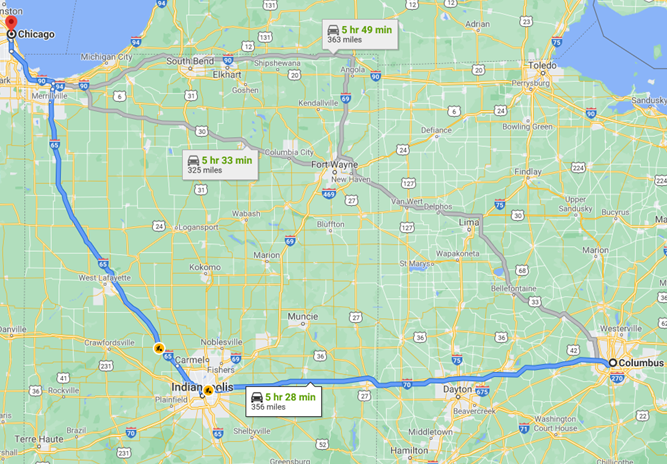
\includegraphics{ColumbusChicago.png}
%\end{image}
%
%
%Draw graphs in tikzi when possible.  Here are two.
%
%\begin{image}
%\begin{tikzpicture}
%    \begin{axis}
%        \addplot[samples=200,domain=0.01:8]{ln(x)};
%    \end{axis}
%\end{tikzpicture}
%\end{image}
%
%\begin{image}
%\begin{tikzpicture}
%    \begin{axis}[xlabel=,ylabel=,width=0.75\linewidth,
%                xmin=-5,xmax=5,
%                ymin=-5,ymax=5,
%                xtick={-4,4},
%                ytick={-4,4},
%                clip=false]
%        \addplot[soliddot] coordinates {(0,0)} node[pin=240:{Carl's house}] ;
%        \addplot[soliddot] coordinates {(2, 3)} node[pin=-30:{restaurant}] ;
%        \addplot[soliddot] coordinates {(-3, 2)} node[pin=100:{pet shop}] ;
%        \addplot[soliddot] coordinates {(-2, -4)} node[pin=150:{gas station}] ;
%        \addplot[soliddot] coordinates {(3, -3)} node[pin=120:{bar}] ;
%        \addplot[mark=none] coordinates {(5, 0)} node[above left] {east};
%        \addplot[mark=none] coordinates {(-5, 0)} node[above right] {west};
%        \addplot[mark=none] coordinates {(0, 5)} node[below right] {north};
%        \addplot[mark=none] coordinates {(0, -5)} node[above right] {south};
%    \end{axis}
%\end{tikzpicture}
%\end{image}
%
%
%You can also add Desmos interactives.  Create them in a Desmos account (I think we have an OSU one.  We should look into that!).  Save them.  Then pull the graph number out of the url.
%\begin{center}  
%\desmos{lxllnpdi6w}{800}{600}  
%\end{center}
%
%%\typeout{************************************************}
%%\typeout{Online Features}
%%\typeout{************************************************}
%
%\section{Online Features}
%
%To add a url, use the link command.
%For more about formatting in Ximera see \link[this url]{https://ximera.osu.edu/intro/gettingStarted/graphicsAndVideos/graphicsAndVideos}.
%
%
%You can also embed \link[YouTube]{https://www.youtube.com/} videos.
%\begin{center}
%\youtube{0aQpLSu2fMs}
%\end{center}
%
%
%
%
%
%\newpage
%
%%\typeout{************************************************}
%%\typeout{Overviews}
%%\typeout{************************************************}
%
%\section{Overviews}
%
%Each Unit has an overview with the organization and learning objectives
%
%\begin{overview}
%\item Generally a folder %(author if relevant)
%	\begin{enumerate}
%	\item some stuff covered in these sections
%		\textit{a subtopic} 
%		\textit{another subtopic} 
%	\item More stuff	
%	\end{enumerate}	
%\item Another Folder 
%	\begin{enumerate}	
%	\item Stuff 
%	\end{enumerate} 
%\end{overview}
%
%
%\begin{objectives}
%\item Learning Objectives Category (Course level learning objective)
%	\begin{itemize}
%	\item more specific goal
%	\item another one 
%	\end{itemize}
%\item Another Category
%	\begin{itemize}
%	\item Linear 
%	\item Parabolas 
%	\item Polynomials 
%	\end{itemize}
%\end{objectives}
%
%
%
%
%\newpage
%
%%\typeout{************************************************}
%%\typeout{Homeworks}
%%\typeout{************************************************}
%
%\section{Homework}
%Each homework problem should be it's own file.  Then the homework is put together using an exerciselist file.  See a Unit 1 folder for an example.  Be sure to keep all the same conventions, just changing the actual problem.  
%
%Some Ximera problem types are available \link[in the footnote]{https://ximera.osu.edu/intro/gettingStarted/questionAndAnswerTypes/questionAndAnswerTypes}.  We can add more here as we come across them.

\end{document}
